\documentclass[a4paper,10pt]{report}
\usepackage[T1]{fontenc}
\usepackage{titlesec}
\usepackage{graphicx}
\usepackage{svg}
\usepackage{amsmath}
\usepackage{amsthm}
\usepackage{fancyvrb}
\usepackage[english]{babel}
\usepackage{csquotes}
\usepackage{hyperref}
\hypersetup{
   colorlinks=true,
   linkcolor=blue,
   urlcolor=cyan
}
\usepackage{tikz}
\usepackage{amssymb}
\usepackage{palatino}
\usepackage{breqn}
\usepackage{caption}
\usepackage{subcaption}
\usepackage{minted}
\setminted{
   numberblanklines=false, 
   mathescape, 
   texcomments, 
   autogobble, 
   breakanywhere, 
   breakautoindent, 
   breaklines,
   frame=none
}
\setminted[python]{python3}
\usepackage[
   backend=biber,%
   bibencoding=utf8,%
   language=english,%
   style=numeric-comp,%
   sorting=nyt,%
   maxbibnames=10,%
   natbib=true%
]{biblatex}
\addbibresource{references.bib}
\graphicspath{ {./img/} }

% Set TOC depth and sections numbering
\setcounter{tocdepth}{3}
\setcounter{secnumdepth}{3}

% Remove chapters head
\titleformat{\chapter}[display]
  {\normalfont\bfseries}{}{0pt}{\Large}

% Make quotes italic 
\renewcommand{\mkbegdispquote}[2]{\itshape}


\begin{document}
\frenchspacing

% First page
\title{
	{{\large{\textsc{Alma Mater Studiorum $\cdot$ University of Bologna}}}}
	\rule{\textwidth}{0.4pt}\vspace{3mm}
	\textbf{Flatland Challenge} 
	\begin{figure}[!htb]
		\centering
		\includesvg[width = 200pt]{flatland-logo}
	\end{figure} \\
	Deep learning course final project
}

\author{Leonardo Calbi (\href{mailto:leonardo.calbi@studio.unibo.it}{leonardo.calbi@studio.unibo.it}) \\ Alessio Falai (\href{mailto:alessio.falai@studio.unibo.it}{alessio.falai@studio.unibo.it})}
\date{\today}
\maketitle
\newpage
\tableofcontents
\listoffigures
\newpage


\chapter*{Foreword}
The Flatland challenge is a competition organized by AIcrowd \cite{aicrowd} with the help of SBB (Swiss Federal Railways) to foster innovation with what regards the scheduling of trains trajectories in a railway environment. 

As reported on the official challenge website, SBB operates the densest mixed railway traffic in the world. It maintains and operates the biggest railway infrastructure in Switzerland. Today, there are more than $10000$ trains running each day, being routed over $13000$ switches and controlled by more than $32000$ signals. 

The Flatland challenge aims to address the vehicle rescheduling problem by providing a simplistic grid world environment and allowing for diverse solution approaches. In particular, the first edition of the challenge was hosted during 2019 and the submitted solutions were mainly based on OR (Operation Research) methodologies, while the second edition of the competition, i.e. the NeurIPS 2020 edition, had the goal of favoring the implementation of RL (Reinforcement Learning) based solutions.  


\chapter{Introduction}
At the core of this challenge lies the general vehicle re-scheduling problem (VRSP) proposed \citeauthor{vrsp} in \citeyear{vrsp} \cite{vrsp}:
\begin{displayquote}
	The vehicle rescheduling problem (VRSP) arises when a previously assigned trip is disrupted. A traffic accident, a medical emergency, or a breakdown of a vehicle are examples of possible disruptions that demand the rescheduling of vehicle trips. The VRSP can be approached as a dynamic version of the classical vehicle scheduling problem (VSP) where assignments are generated dynamically.
\end{displayquote}

The problem is formulated as a 2D grid environment with restricted transitions between neighboring cells to represent railway networks. On the 2D grid, multiple agents with different objectives must collaborate to maximize the global reward.

The overall goal is to make all agents (trains) arrive at their target destination with a minimal travel time. In other words, we want to minimize the time steps (or wait time) that it takes for each agent in the group to reach its destination.


\chapter{Background}
As already pointed out, the Flatland environment is represented as a 2D grid and each cell can be one of many different types. The different types of cells can belong to the following categories: \texttt{rail}, \texttt{target} and \texttt{empty}.

About the \texttt{target} cells, they represent the destination of one or more agents (different agents could have the same target) and the number of possible targets present in the environment is clearly limited by the number of agents.

The \texttt{rail} cells are more intricated, in that there exists different types of them. In particular, figure \ref{fig:rail-cells} shows examples of possible \texttt{rail} cells that can be used to build up a railway environment in Flatland. Other than the ones shown in figure \ref{fig:rail-cells} there are also diamond crossings (i.e. two orthogonal straight rails crossing each other), single slip switches (i.e. the same as double slip switches but with a single choice) and symmetrical switches (which are special kinds of switches that bifurcate to a left and right branch). Moreover, every \texttt{rail} cell can be rotated by $90^{\circ}$ and mirrored along both axis.

An important fact about the different types of \texttt{rail} cells is that only switches require an agent to make a choice. In Flatland (like in reality) a maximum of two options is available. There does not exist a switch with three or more options.

\begin{figure}[h]
	\centering
	\captionsetup[subfigure]{justification=centering}
	\begin{subfigure}[t]{.25\linewidth}
		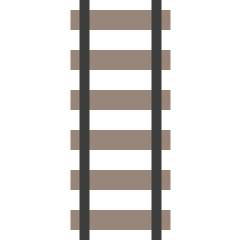
\includegraphics[width=\textwidth]{straight-rail.png}
		\caption{Straight}
		\label{fig:rail-cells-straight}
	\end{subfigure}%
    ~
	\begin{subfigure}[t]{.25\linewidth}
		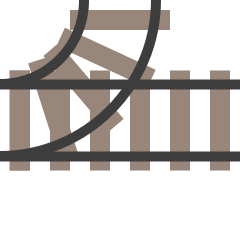
\includegraphics[width=\textwidth]{simple-switch-rail.png}
		\caption{Simple switch}
		\label{fig:rail-cells-simple}
	\end{subfigure}%
	~ 
	\begin{subfigure}[t]{.25\linewidth}
		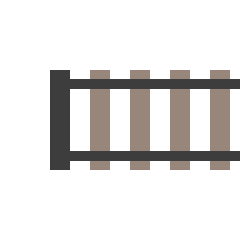
\includegraphics[width=\textwidth]{deadend-rail.png}
		\caption{Deadend}
		\label{fig:rail-cells-deadend}
	\end{subfigure}%
	~
	\begin{subfigure}[t]{.25\linewidth}
		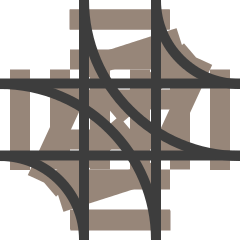
\includegraphics[width=\textwidth]{double-slip-rail.png}
		\caption{Double slip switch}
		\label{fig:rail-cells-double}
	\end{subfigure}%
    
	\caption{Different \texttt{rail} cell types}
	\label{fig:rail-cells}
\end{figure}

Finally, every cell that is not \texttt{rail} or \texttt{target} is \texttt{empty}. As shown in figure \ref{fig:env-example}, it is interesting to notice that Flatland is a very sparse environment, meaning that there are a lot more \texttt{empty} cells than non-\texttt{empty} ones: because of this, representing the environment as a simple dense matrix could lead to overheads and efficiency issues, especially when dealing with relatively big environments.

\begin{figure}[h]
	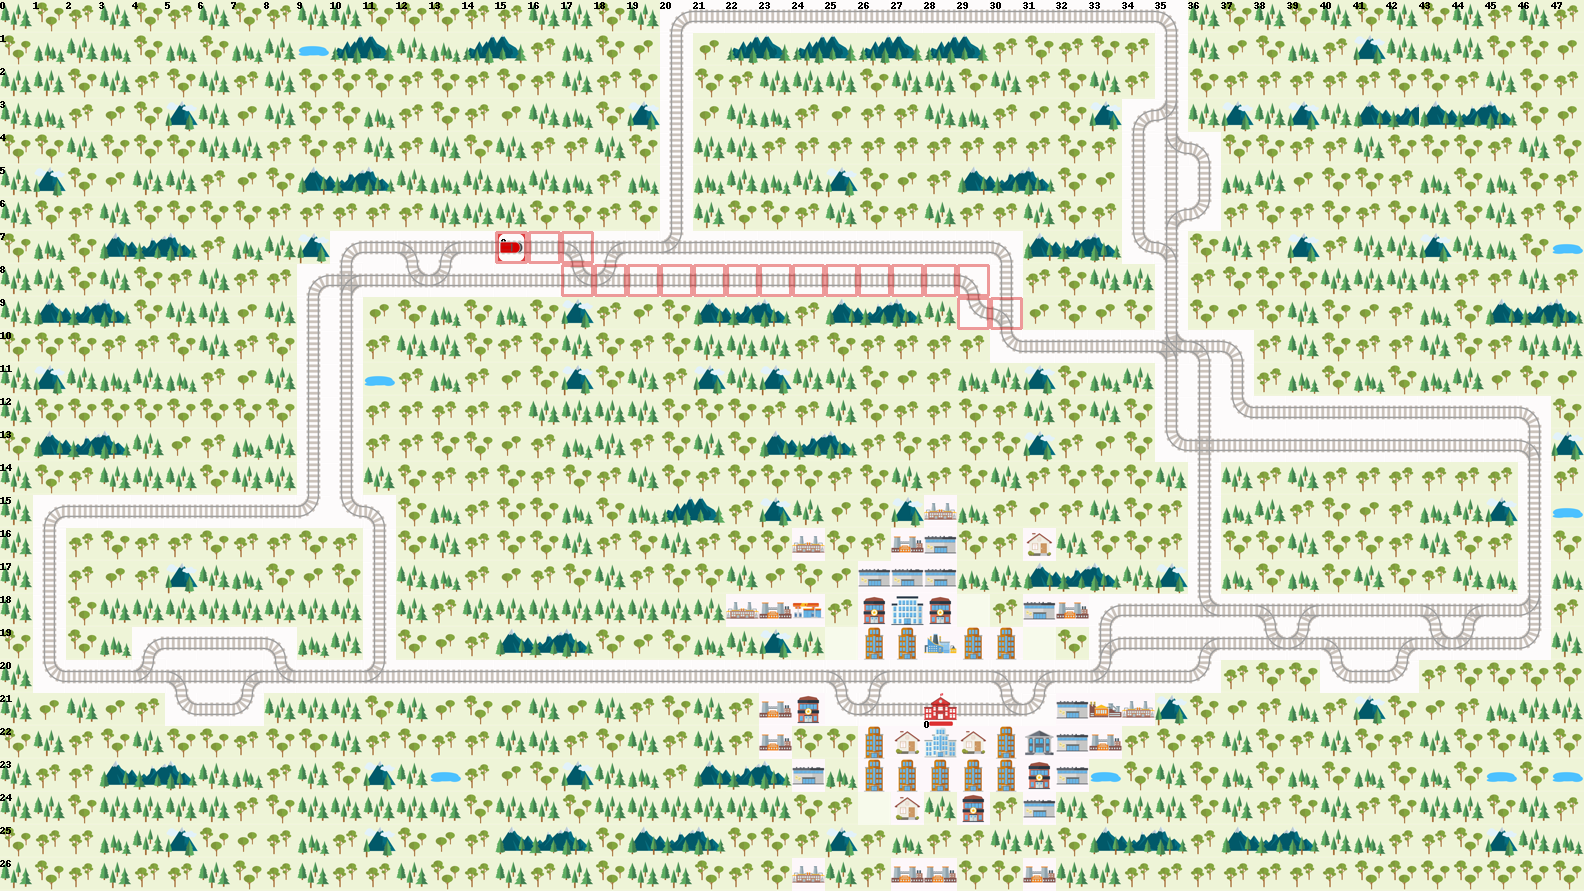
\includegraphics[width=\textwidth]{env.png}
	\caption{An example of a railway environment}
	\label{fig:env-example}
\end{figure}

An agent in the Flatland environment is a train that starts from a random \texttt{rail} cell in the map and has to arrive to its assigned \texttt{target} cell. To do so, the agent can only occupy \texttt{rail} and \texttt{target} cells. To move from a cell to another one the agent has to make a choice and, depending on the cell type that they are on

Each \texttt{rail} cell 

Flatland has a discrete action space, meaning that only $5$ possibilities have to be considered at each transition. In particular, Flatland considers the following actions:
\begin{enumerate}
	\item \texttt{MOVE_FORWARD}
	\item \texttt{MOVE_LEFT}
	\item \texttt{MOVE_RIGHT}
	\item \texttt{STOP_MOVING}
	\item \texttt{DO_NOTHING}
\end{enumerate}


\chapter{Environment}
\section{Railway encoding}
\section{Observations}
\subsection{Tree}
\subsection{Binary tree}
\section{Predictions}
\subsection{Shortest path}
\section{Choices}
\section{Rewards shaping}

\chapter{Policy}
\section{Action masking}
\section{Action selection}
\subsection{$\epsilon$-greedy}
\subsection{Boltzmann}
\section{Replay buffers}
\subsection{Uniform}
\subsection{Prioritized}

\chapter{DQN}
\section{Architectures}
\subsection{Vanilla}
\subsection{Double}
\subsection{Dueling}
\section{Bellman equation}
\subsection{Max}
\subsection{Softmax}

\chapter{GNN}

\chapter{Results}



\chapter{Conclusions}

\printbibliography

\end{document}
